\subsection{Medical Services Crew}

The Medical Services Crew operates follows a \textbf{sequential} task structure to plan the treatment and evacuation of injured people from the emergency site. The tasks included within the Medical Services are:

\begin{enumerate}
	\item \textbf{Receive Report:} The \textit{Medical Services Operator} receives the fire incident report, and parses key information, such as the location, the number of injured, and the severity of injuries.

	\item \textbf{Assess Hospital Capacity:} The \textit{Hospital Coordinator} assesses the available resources (beds, ambulances, paramedics) at their respective hospital, and reports how much they can supply. This task depends on the completion of the \textit{Recieve Report} task.
	
	\item \textbf{Deploy Paramedics:} Based on the location and the assigned resources to the emergency, \textit{Paramedics} are deployed to the place of the incident, reporting an estimation of the time of arrival and a list of the medical procedures that will have to be performed. This task depends on the completion of both the \textit{Recieve Report} and the \textit{Assess Hospital Capacity} tasks.
	
	\item \textbf{Report Medical Response:} The \textit{Medical Services Operator} reports back a comprehensive summary of the response plan, along with important information, such as whether all the medical needs of the emergency can be fully supplied by its hospital or not. This task depends on the completion of the \textit{Assess Hospital Capacity} and \textit{Deploy Paramedics} tasks.
\end{enumerate}

\textcolor{red}{Remove task dependencies from here. Put the figure after task dependencies. Also, make figure for Medical Services}

\begin{figure}[h!]
	\centering
	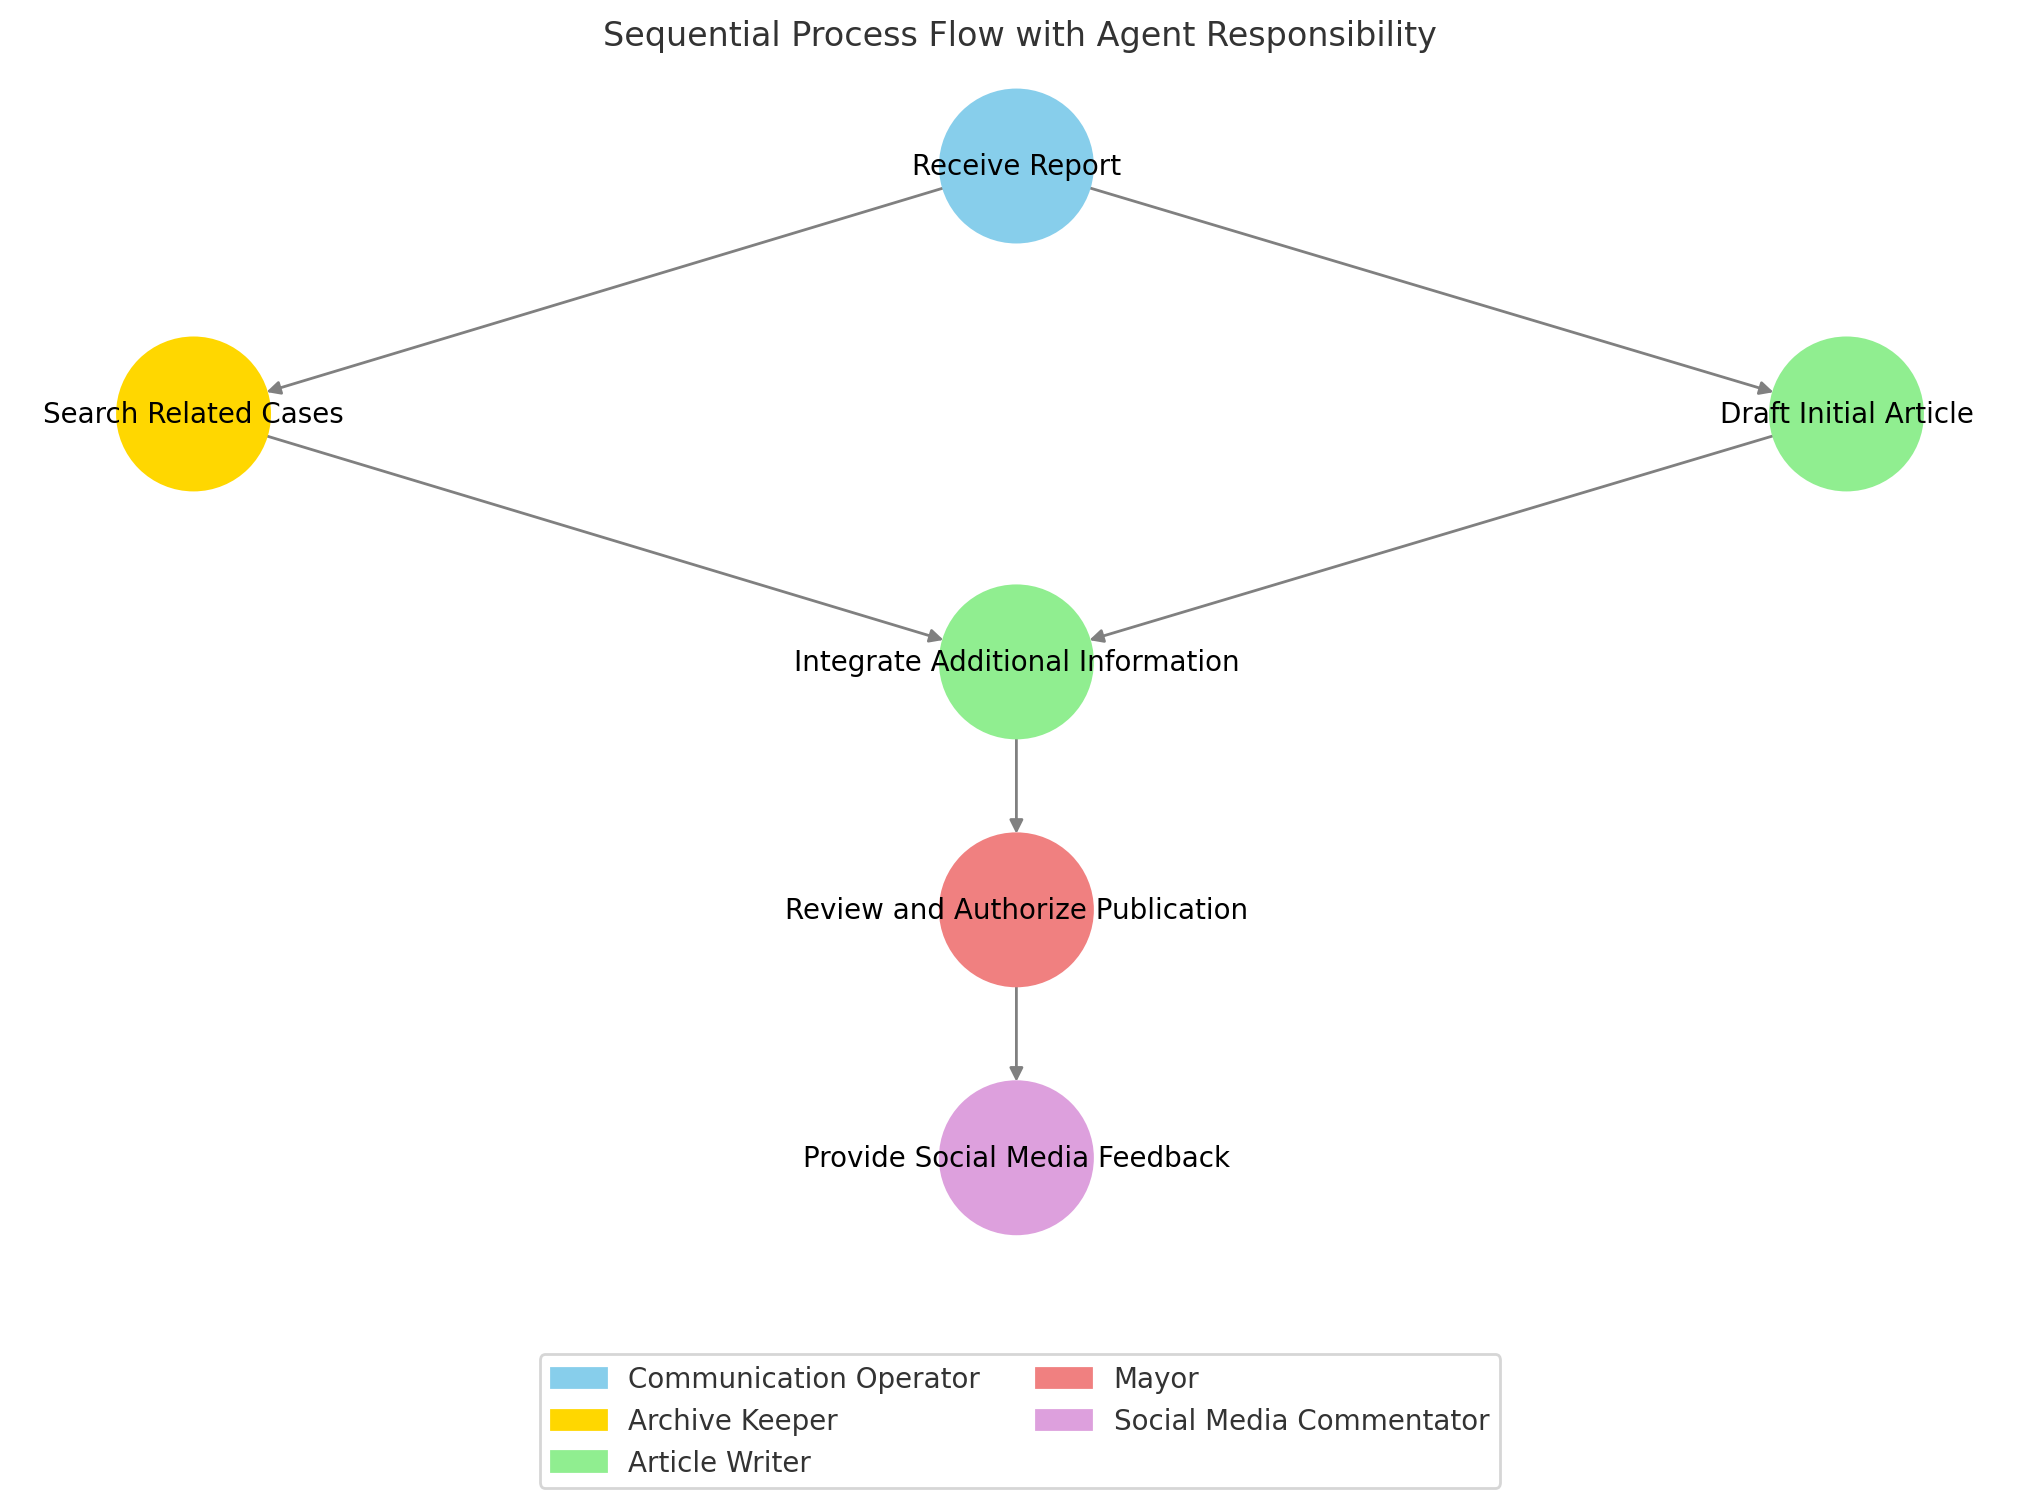
\includegraphics[width=0.9\textwidth]{figures/PC-process.png}
	\caption{Sequential Process Flow of the Medical Services Crew with Agent Responsibilities}
	\label{fig:medical_services_flow}
\end{figure}


\paragraph{Task Dependencies}
The sequential nature of the process requires to establish task dependencies to define the crew's workflow:
\begin{itemize}
	\item 
\end{itemize}

The task dependencies and agents who perform each task can be observed in Figure~\ref{fig:medical_services_flow}.
